\section{Sprint 2}
Der zweite Sprint baut auf den Arbeiten des ersten auf.
So wird eine Story welche im ersten Sprint begonnen wurden, in diesem abgeschlossen.
Einige Funktionen, welche in Sprint 1 entwickelt wurden, werden in Sprint 2 zusammengeführt und erweitert.
Konkret werden diesen Stories bearbeitet:
\begin{itemize}
   \item Die Applikation soll auf \ac{ADO} bei jedem neuem Commit automatisch gebaut und getestet werden. 
   \item Werte von Attributen sollen vom Zähler ausgelesen und in der Benutzerschnittstelle dargestellt werden.
   \item Die Benutzerschnittstelle soll das Schreiben von Attributwerten sowie ausführen von Methoden unterstützen.
\end{itemize}


\subsection{Build bei Commit}\label{s2:buildOnCommit}
Die Arbeiten an dieser Story wurden bereits im vorherigen Sprint begonnen.
Das Ziel der Story und das bisherige Vorgehen ist im Abschnitt \ref{story_buildoncommit} aufgeführt.
Die Pipeline in \ac{ADO} wurde nun so konfiguriert, dass die Solution kompiliert wird.
Dies funktionierte problemlos.
Als die Pipeline um einen Task erweitert wurde, welcher die Tests ausführen soll traten Schwierigkeiten auf.
Im Log war der Fehler \dq  Could not find testhost\dq , ausgelöst von \textit{vstest.console.exe}, zu lesen.
Da die Unit-Tests lokal jeweils über Visual Studio ausgeführt wurde, trat dieser Fehler dort nicht auf.
Er konnte jedoch reproduziert werden, indem \textit{vstest.console.exe} gleich wie bei der Pipeline aufgerufen wurde.
Ein Test mit einem neuen, leeren Projekt, welcher zum gleichen Fehler fürte, zeigte, dass es sich dabei um einen Fehler von Visual Studio handelt muss.

Dieses Problem konnte umgangen werden, indem anstelle von msbuild\footnote{https://docs.microsoft.com/en-us/visualstudio/msbuild/msbuild?view=vs-2022}
die .NET CLI\footnote{https://docs.microsoft.com/en-us/dotnet/core/tools/} für das Kompilieren und Ausführen der Tests verwendet wird.
Bei der Verwendung der .NET CLI trat ein neues Problem auf.
Diese Unterstützt das Kompilieren von WinUI3 Anwendungen nicht.
Da, wie bereits in Abschnitt \ref{objectModelDevSchwierigkeiten} erklärt, bei den Unit-Test gar keine Abhängigkeiten zu WinUi3 bestehen können ist dies nicht weiter tragisch.
Damit das Kompilieren erfolgreich funktioniert, wurde eine zweite Solution erstellt, welche nur jene C\# Projekte enthält, die nicht von WinUI3 abhängen.

So konnte die Story trotz diverser Schwierigkeiten fertiggestellt werden.

\subsection{Lesen von Attributen}
\dq Werte von Attributen sollen vom Zähler ausgelesen und in der Benutzerschnittstelle dargestellt werden.\dq
\subsubsection{Ziel}
Im ersten Sprint wurde die Kommunikation mit den Stromzählern implementiert.
Ebenfalls wurde eine Visualisierung des Object Models zur Benutzerschnittstelle hinzugefügt.
Diese Dinge sollen nun so kombiniert werden, dass im Object Model ein Attribut angewählt werden kann und dieses über einen Klick ausgelesen wird.
Die Werte sollen dabei jeweils direkt im Object Model angezeigt werden.
Die Story gilt als erledigt, wenn Attribute inklusive Arrays und Strukturen korrekt ausgelesen und dargestellt werden können.

\subsubsection{Vorgehen und Schwierigkeiten}\label{readAttributVorgehen}
Für das Auslesen von Attributen kann das \textit{IRawReader} Interface verwendet werden.
Dieses wird von der in Sprint 1 erstellten Klasse \textit{ReaderWriter} implementiert.
Der Methode \textit{Read} wird ein Short Name als Parameter mitgegeben und sie gibt den ausgelesenen Wert als String zurück.
Beim Short Name handelt es sich um eine Kombination aus Objektname und Attributname, welche ein bestimmtes Attribut eindeutig identifiziert.
Die ausgelesenen Werte werden vom \ac{ATS} Code in einem proprietären Format zurückgegeben. 
Dieses sieht beispielsweise wie folgt aus:
\begin{verbatim}
   Struct[3](
      Integer16('0005')
      OctetString[6]('112233445566')
      Integer8('01')
   )'
\end{verbatim}
\begin{figure}
\centering
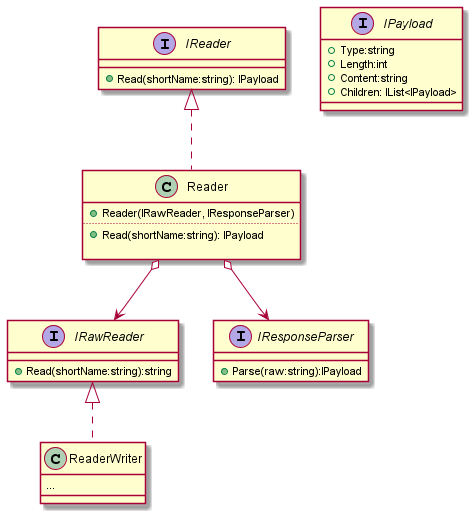
\includegraphics[width=0.7\textwidth]{gfx/string_toPayload.png}
\caption{
   Klassendiagramm zur Reader Klasse
   }
   \label{fig:reader}
\end{figure}
Diese Struktur wurde in der Applikation durch das Interface \textit{IPayload} repräsentiert.
Die Klasse \textit{Reader}, welche im Klassendiagramm \ref{fig:reader} dargestellt ist, liest Werte aus dem Zähler aus und gibt diese als \textit{IPayload} zurück.
So kann in der Applikationslogik vereinfacht gelesen und auf die Antwort zugegriffen werden.

Die Datentypen der Attribute lassen sich in die Kategorien einfach und komplex einteilen.
Zu den einfachen Typen gehören Strings und numerische Typen wie Integer oder Float.
Arrays und Strukturen sind komplexe Typen.
Um einen einfachen Typen in der Benutzeroberfläche darzustellen, reicht eine Textbox aus.
Eine Struktur setzt sich jedoch jeweils aus mehreren Werten zusammen und benötigt deshalb für die Darstellung auch mehrere Textboxen.
Genaue Angaben zu den Typen sind im Object Model nicht vorhanden.
Die Antwort, welche beim Lesen eines Attributs zurückgegeben wird, beinhaltet Angaben zum Aufbau von komplexen Typen.
So ist ihr jeweils zu entnehmen, wie viele Felder eine Struktur enthält oder aus wie vielen Elementen ein Array besteht.
Weiterführende Informationen, wie beispielsweise die Namen der Felder einer Struktur, sind in den Class Descriptions abgelegt.

Wie bereits in Abschnitt \ref{objectModelsClassDescriptions} beschrieben, hat die Landis+Gyr C\# Programme, welche Class Descriptions parsen.
Das C\# Projekt \textit{InfraLib} enthält eine Klassenstruktur, welche Class Descriptions repräsentiert.
Um eine möglichst lose Koppelung zu \textit{InfraLib} zu erreichen, wurden Interfaces für eine eigene Klassenstruktur geschreiben.
Das Adapter Pattern \parencite{designPatterns} wurde eingesetzt, um die Klassen der \textit{InfraLib} mit den eigenen Interfaces zu verbinden.
So konnte jedes Objekt mit seiner Class Description verbunden werden.
Die zusätzlichen Informationen ermöglichen ein einfaches Darstellen von komplexen Typen.
\begin{figure}
   \centering
   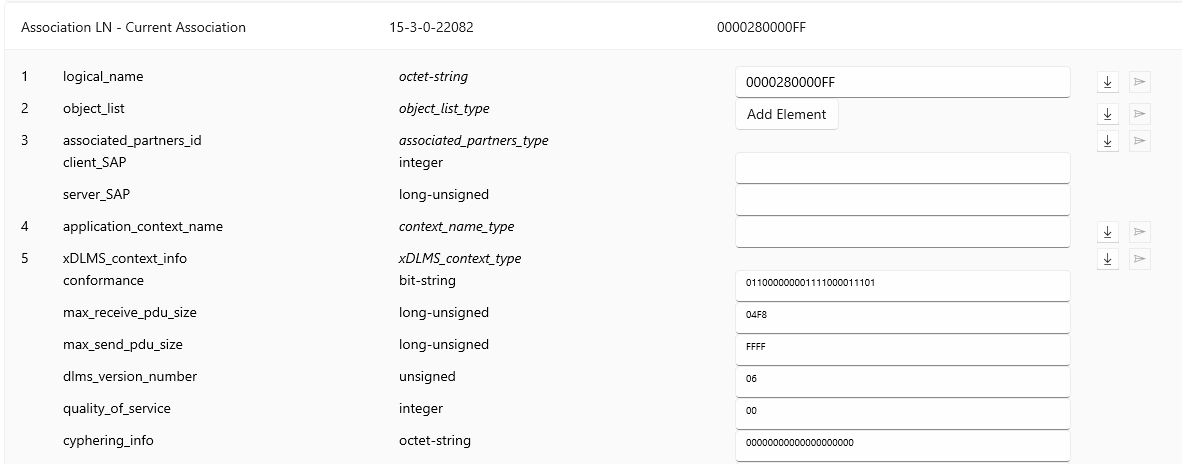
\includegraphics[width=1.0\textwidth]{gfx/AttributeReadExample.png}
   \caption{
      Ausschnitt aus DlmsQuickAccess zum Lesen von Strukturen
      }
      \label{fig:AttributeReadExample}
   \end{figure}
In Abbildung \ref{fig:AttributeReadExample} ist ein Attribut abgebildet, welches ausgelesen wurde.
Dabei ist ersichtlich, dass alle Felder des Struktur \textit{xDLMS\_context\_type} mit Name und Typ beschriftet sind.

Bei der Integration der \textit{InfraLib} in die Solution musste festgestellt werden, dass zwar einige Unit-Tests vorhanden sind, jedoch nur geringe Teile des Codes getestet sind.
Da einige Fehler im Parsing-Code gefunden wurde, wurden einige Modul Tests geschreiben, welche das Zusammenspiel der verschiedenen Komponenten von XML-Files bis Adapter testen.

Der Code der \textit{InfraLib} wurde gleich wie der \ac{ATS} Code eingebunden (siehe Abschnitt \ref{atsUmsetztung}).
Die \textit{InfraLib} in Zukunft als NuGet Paket zu verwenden, wäre jedoch mit weniger Aufwand verbunden als beim \ac{ATS}, da diese bereits als Library aufgebaut ist.

\subsection{Schreiben von Attributen}
\dq Die Benutzerschnittstelle soll das Schreiben von Attributwerten sowie Ausführen von Methoden unterstützen.\dq

\subsubsection{Ziel}
In der vorherigen Story wurde das Lesen von Attributen über die Benutzerschnittstelle implementiert.
Ziel dieser Story ist es, dass über die selbe Schnittstelle Schreibbefehle ausgeführt werden können.
Ebenfalls soll es möglich sein, dass Methoden ausgeführt werden können.

\subsubsection{Vorgehen und Schwierigkeiten}
Um nebst dem Lesen auch das Schreiben von Attributen über die Benutzerschnittstelle steuern zu können mussten entsprechende \textit{Button} Controls hinzugefügt werden.
Die meisten bestehenden Komponente wurden bereits zuvor so entwickelt, dass sie das Schreiben ebenfalls unterstützen.
In Text zur vorgehenden Story wurde beschreiben, wie das Datenformat des \ac{ATS} Codes in eine eigene Klassenstruktur überführt wurde.
Um Daten zu schreiben, musste dieser Prozess umgekehrt werden.

\begin{figure}
   \centering
   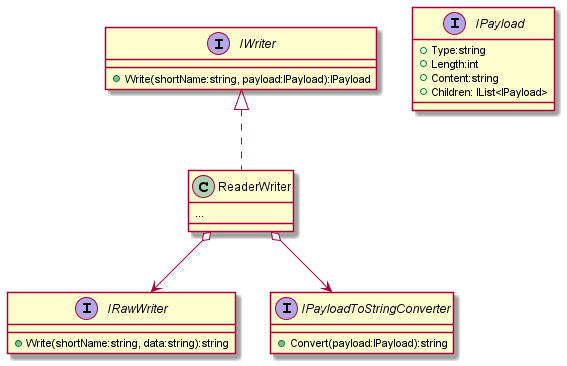
\includegraphics[width=1.0\textwidth]{gfx/payloadTostriing.png}
   \caption{
      Klassendiagramm zur Writer Klasse
      }
      \label{fig:writer}
   \end{figure}
Dies wurde mit der \textit{Writer} Klasse, welche in Abbildung \ref{fig:writer} aufgezeigt ist, implementiert.


Das Ausführen von Methoden funktioniert technisch gleiche wie das Schreiben von Attributen.
Die Parameter der Methode werden dazu als Schreib-Payload mitgegeben.
So kann die \textit{Writer} Klasse auch für das Ausführen von Methoden verwendet werden.
Die Darstellung der Methoden in der Benutzeroberfläche musste um Eingabefelder für die Parameter und ein \textit{Button} Control für das Starten der Ausführung ergänzt werden.
Dabei konnten Element wiederverwendet werden, welche auch bei den Attributen eingesetzt werden.
\begin{figure}
   \centering
   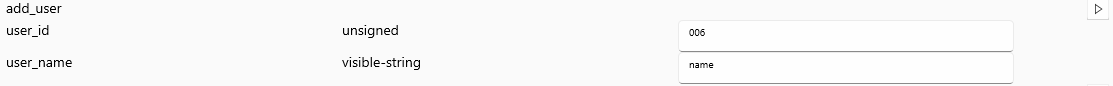
\includegraphics[width=1.0\textwidth]{gfx/addUserMethod.png}
   \caption{
      Ausschnitt aus DlmsQuickAccess der Methode add\_user
      }
      \label{fig:addUserMethod}
   \end{figure}



\subsection{Integrationstests}
Während dieses Sprints musste oft die ganze Anwendung gestartet werden, um die neue Funktionen zu testen.
Deshalb wurde für die Validation der Stories dieses Sprints erste Integrationstests geschrieben.
Diese sind so aufgebaut, dass bis auf die Benutzerschnittstelle alle Teile der Applikation inklusive Kommunikation mit den Stromzählern aufgesetzt und verschiedene Aktionen ausgeführt werden.
Es wird also das Zusammenspiel der ViewModels mit dem Model getestet.

\subsection{Erster richtiger Release}\label{firstRelease}
Bereist ein Arbeitstag vor Sprintende waren alle geplanten Stories fertiggestellt.
Da die Applikation bereits erste Funktionalität beinhaltet, wurde diese veröffentlicht und den Nutzern in einer Demo präsentiert.
Die Resonanz dabei war positiv.
Der Release beinhaltete jedoch noch einige Limitierungen.
So wird beispielsweise nur ein spezifisches Version eines einzigen Produktes, \textit{Ref\_MMI3}, unterstützt.
Als erste Benutzer den DlmsQuickAccess installierten und starteten, stürzte dieser direkt ab.
Im nächsten Sprint sollen diese Abstürze untersucht, sowie die Unterstützung von weiteren Produkttypen sichergestellt werden.
